\documentclass[12pt, a4paper, twoside]{article}
\usepackage[utf8]{inputenc}
\usepackage[english]{babel}
\usepackage[T1]{fontenc}
\usepackage[margin=2cm]{geometry}
\usepackage{amsmath}
\usepackage{amsfonts}
\usepackage{amssymb}

%% Fonts
\usepackage{lmodern}
%\usepackage{mathptmx} % Times New Roman
%\usepackage{fouriernc}
%\usepackage{newpxtext, newpxmath} % Palatino

\usepackage{indentfirst} % paragraph after title
\usepackage{siunitx} % SI units
\usepackage[bookmarks, hidelinks]{hyperref} % links for sections
\usepackage{graphicx}
\usepackage{float}
\usepackage{esdiff}
\usepackage{fancyhdr}
\usepackage[nodayofweek,level]{datetime}

\numberwithin{equation}{section} % number equations by section
\graphicspath{{figures/}}

%% Fancy Header - page number at the right side of the page
\lhead{} \chead{} \rhead{} %sets header left center right
\lfoot{} \cfoot{} \rfoot{\thepage} %sets footer left center right
\renewcommand{\headrulewidth}{0.0pt} %optional horizontal rule thickness
\renewcommand{\footrulewidth}{0.0pt} %optional horizontal rule thickness
\pagestyle{fancy}

\title{Computational Heat Transfer and Fluid Mechanics - Problem 1}
\author{Guilherme Gwadera}
\date{\today}



\begin{document}

%\newgeometry{margin=2cm}
\begin{titlepage}

\centering

\includegraphics[width=0.4\textwidth]{brasao.eps} \par
%\vspace{1cm}
\textsc{\large{Centro Tecnológico \\ Departamento de Engenharia Mecânica}}
\par
\vspace{1cm}
\textsc{\large{EMC 5412 -- Transferência de Calor e \\ Mecânica dos Fluidos Computacional}}
\par
\vspace{0.25cm}
\textsc{\large{Professor Antonio Fábio Carvalho da Silva}}
\par
\vspace{1.5cm}
\par
\LARGE{\textbf{Thermal Conductivity Evaluation\\at an Interface}}
\par
\vspace{2cm}
\textsc{\large{Guilherme Gwadera}}
\par
\vfill
\textsc{\large{Florianópolis, \formatdate{30}{8}{2018}}}
\par
\end{titlepage}
%\restoregeometry
\section{Introduction}

The proposed problem consists of a wall composed by two materials of different thermal conductivities, with a prescribed heat flow $q'' =$ \SI{6000}{W/m^2} on the left border, and a convective heat flow on the right border, with $h =$ \SI{100}{W/m^2.K} and $T_\infty =$ \SI{40}{\celsius}.
For this case, steady state is assumed.

\begin{figure}[h]
    \centering
    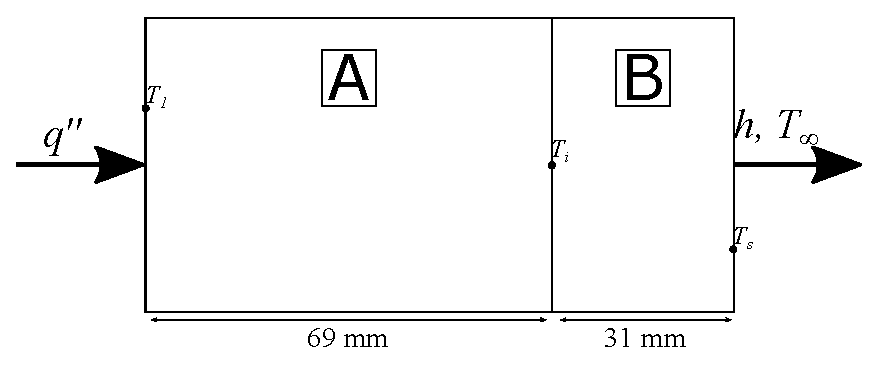
\includegraphics[scale=1]{problema.eps}
    \caption{Schematic representation of the problem.}
    \label{fig:problema}
\end{figure}

By making an energy balance at the borders and at the contact interface, the exact values of the analytical solution of the problem are easily found:

\begin{equation*}
    q'' = \frac{k_A \left(T_1 - T_i \right)}{L_A} = \frac{k_B \left(T_i - T_s \right)}{L_B} = h \left(T_s - T_\infty \right)
\end{equation*}

\begin{equation*}
    \SI{6000}{W/m^2} =
    \frac{10 \left(T_1 - T_i \right)}{0,069} =
    \frac{1  \left(T_i - T_s \right)}{0,031} =
    100 \left(T_s - 40 \right)
\end{equation*}

\begin{align*}
    T_1 &= \SI{327.4}{\celsius} \\
    T_i &= \SI{286}{\celsius} \\
    T_s &= \SI{100}{\celsius}
\end{align*}

For the numerical solution of the temperature profile, it is necessary to discretize the differential equation obtained by an energy balance (Equation \ref{eq:eqdif}), also applying the two boundary conditions (Equations \ref{eq:cc1} and \ref{eq:cc2}).

\begin{align} 
    \diff{}{x} \left( k \diff{T}{x} \right) &= 0 \label{eq:eqdif} \\
    -k \left. \diff{T}{x} \right|_{x = 0} &= q'' \label{eq:cc1} \\
    -k \left. \diff{T}{x}\right|_{x = L} &= h \left(T_s - T_\infty \right) \label{eq:cc2}
\end{align}

Discretizing the domain in $N_A$ control volumes for the $A$ part and $N_B$ control volumes for the $B$ part, placing the mesh points at the domain boundaries, a mesh is obtained as in the figure \ref{fig:mesh}.
The points in the $A$ part are separated by a distance $\delta x_A$ and the points in the $B$ part are separated by a distance $\delta x_B$, calculated according to the equations below:

\begin{equation*}
    \delta x_A = \frac{L_A}{N_A - 0,5} \qquad\qquad \delta x_B = \frac{L_B}{N_B - 0,5}
\end{equation*}

\begin{figure}[h]
    \centering
    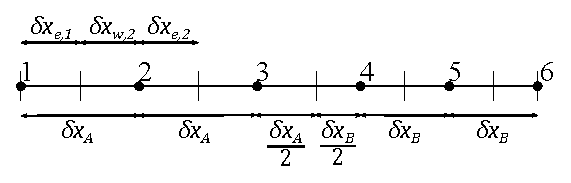
\includegraphics[scale=1.2]{mesh.eps}
    \caption{Schematic representation of the mesh.}
    \label{fig:mesh}
\end{figure}

For points within the mesh, the discretization by the finite volume method for an arbitrary point $P$, in this case called $i$ is given by the equations below, with point $i + 1$ equivalent to point $E$ (East), and the $i-1$ point equivalent to the $W$ (West) point:

\begin{align*}
    a_p T_P &= a_e T_E + a_w T_W \\
    a_i T_i &= a_{i+1} T_{i+1} + a_{i-1} T_{i-1} \\
    a_e &= a_{i+1} = \frac{k_e A}{\delta x} = \frac{k_e A}{\delta x_{e,i} + \delta x_{w,i+1}} \\
    a_w &= a_{i-1} = \frac{k_w A}{\delta x} = \frac{k_w A}{\delta x_{w,i} + \delta x_{e,i-1}}\\
    a_p &= a_i = a_{i+1} + a_{i-1}
\end{align*}

Where $k_e$ and $k_w$ for neighboring volumes with different thermal conductivities are calculated by linear variation or by the formulation of thermal resistances:

\begin{align*}
    k_{e, \text{linear}} &= f_e k_P + (1 - f_e) k_E = f_e k_i + (1 - f_e) k_{i+1} \\
    k_{e, \text{resistances}} &= \left(\frac{1 - f_e}{k_P} + \frac{f_e}{k_E} \right)^{-1} = \left(\frac{1 - f_e}{k_i} + \frac{f_e}{k_{i+1}} \right)^{-1} \\
    f_e &= \frac{\delta x_{w,E}}{\delta x} = \frac{\delta x_{w,i+1}}{\delta x_{w,i+1} + \delta x_{e,i}} \\
    k_{w, \text{linear}} &= f_w k_P + (1 - f_w) k_W = f_w k_i + (1 - f_w) k_{i-1} \\
    k_{w, \text{resistances}} &= \left(\frac{1 - f_w}{k_P} + \frac{f_w}{k_W} \right)^{-1} = \left(\frac{1 - f_w}{k_i} + \frac{f_w}{k_{i-1}} \right)^{-1} \\
    f_w &= \frac{\delta x_{e,W}}{\delta x} = \frac{\delta x_{e,i-1}}{\delta x_{e,i-1} + \delta x_{w,i}}
\end{align*}

For the first boundary condition (prescribed heat flux), applying finite volume discretization and integrating the differential equation, an algebraic equation is obtained as follows:

\begin{align*}
    a_p T_P &= a_e T_E + b \\
    a_1 T_1 &= a_2 T_2 + b \\
    a_p &= a_e = \frac{k_e A}{\delta x} = \frac{k_e A}{\delta x_{e,1} + \delta x_{w,2}} \\
    b &= q'' A = 6000
\end{align*}

For the second boundary condition, the discretized equation is obtained in the same way, arriving at the equations shown below, where $N$ is the last point of the mesh ($N = N_A + N_B$).

\begin{align*}
    a_p T_P &= a_w T_W + b \\
    a_N T_N &= a_{N-1} T_{N_1} + b \\
    a_w &= \frac{k_w A}{\delta x} = \frac{k_w A}{\delta x_{e,N-1} + \delta x_{w,N}} \\
    a_p &= a_w + h A \\
    b &= h A T_\infty = 4000
\end{align*}

With all the equations discretized, a $N \times N$ matrix is constructed with the linear coefficients $a_p$, $a_e$ and $a_w$ for each point of the mesh in each line of the matrix, thus generating a tri-diagonal matrix.
From the two boundary conditions, the column matrix of independent terms of the linear system is constructed, given by the prescribed heat flow and the convective coefficient with its respective external fluid temperature.
Then, the system of equations can be solved using the internal \emph{MATLAB} algorithms, finding the temperatures at each point in the mesh.
As an example, for the mesh represented in Figure \ref{fig:mesh}, the system of equations is:

\begin{equation*}
    \begin{bmatrix}
             362,3188 & -362,3188 &         0 &         0 &         0 &         0  \\
            -362,3188 &  724,6377 & -362,3188 &         0 &         0 &         0  \\
                    0 & -362,3188 &  494,2450 & -131,9261 &         0 &         0  \\
                    0 &         0 & -131,9261 &  212,5713 &  -80,6452 &         0  \\
                    0 &         0 &         0 &  -80,6452 &  161,2903 &  -80,6452  \\
                    0 &         0 &         0 &         0 &  -80,6452 &  180,6452
    \end{bmatrix}
    \cdot
    \begin{bmatrix}
        T_1 \\
        T_2 \\
        T_3 \\
        T_4 \\
        T_5 \\
        T_6
    \end{bmatrix}
    =
    \begin{bmatrix}
        6000 \\
        0 \\
        0 \\
        0 \\
        0 \\
        4000
    \end{bmatrix}
\end{equation*}
\section{Results}

Using the mesh of Figure \ref{fig:mesh}, that is, dividing the domain into 6 volumes (3 for each material), the resulting temperature profile is the one shown in Figure \ref{fig:6points}.
It should be noted that when evaluating the conductivity at the interface using the resistance method, the temperature values obtained are the same as the exact solution.
However, by assessing conductivity by linear variation, temperatures in material A are underestimated.
As the exact solution of the problem already has a linear behavior, and as the finite volume method is conservative, the discretization of the equations with the conductivity evaluated by the resistances method is equivalent to the analytical equations.
Therefore, using this method to calculate the thermal conductivity at the interface, the result will always be the exact one for this specific case, and without being influenced by the mesh size.

\begin{figure}[H]
    \centering
    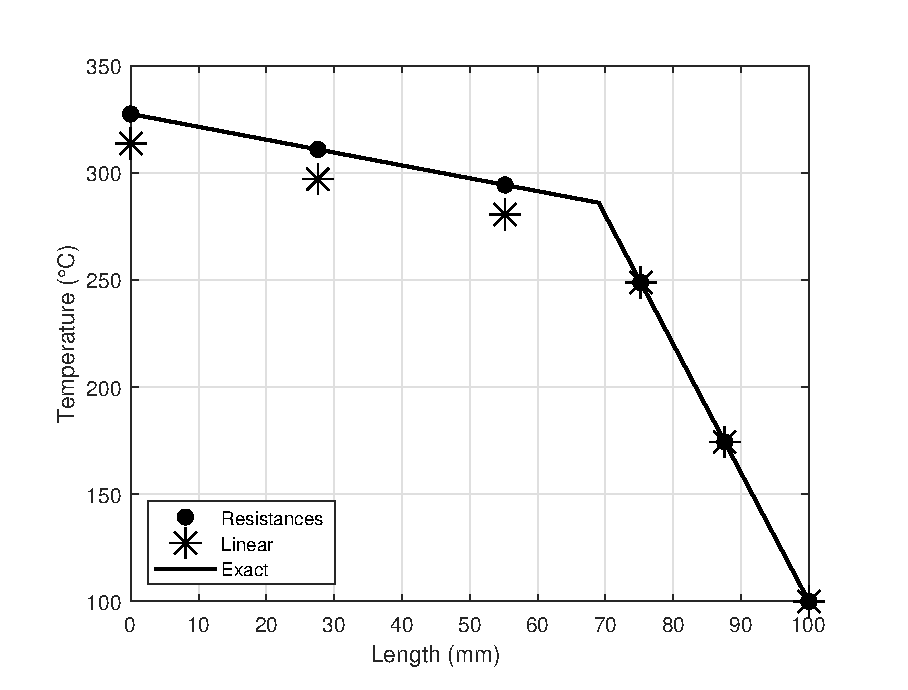
\includegraphics[scale=0.8]{6points.eps}
    \caption{Temperature profile with 6 control volumes in total.}
    \label{fig:6points}
\end{figure}

When increasing the number of control volumes to 20, with 10 volumes in each material, the temperature profile obtained is that of Figure \ref{fig:20points}.
It can be seen that the temperatures with the linear assessment of conductivity at the interface tend to approximate the exact result when refining the mesh.
This result is logical, since by decreasing the thickness of the control volumes, the calculation of the conductivity by linear variation becomes increasingly closer to the real value.
This behavior can be seen in Figure \ref{fig:error}, in which the absolute temperature error $T_1$ tends to be null, however, after a $N$ of about 40 volumes, the error decreases at a very fast rate in relation to the number of volumes.

\begin{figure}[H]
    \centering
    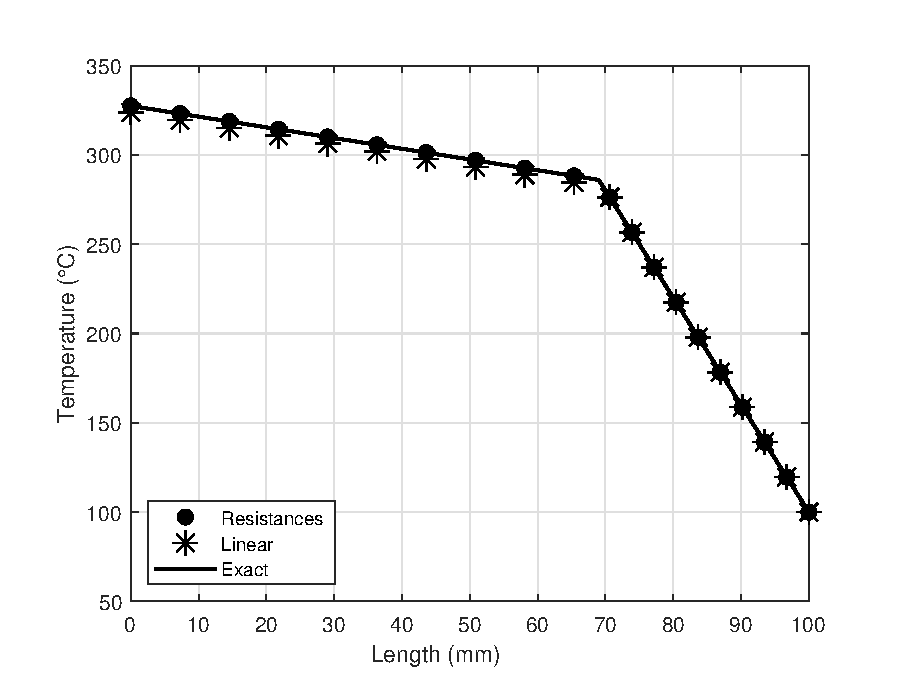
\includegraphics[scale=0.8]{20points.eps}
    \caption{Temperature profile with 20 control volumes in total.}
    \label{fig:20points}
\end{figure}

\begin{figure}[H]
    \centering
    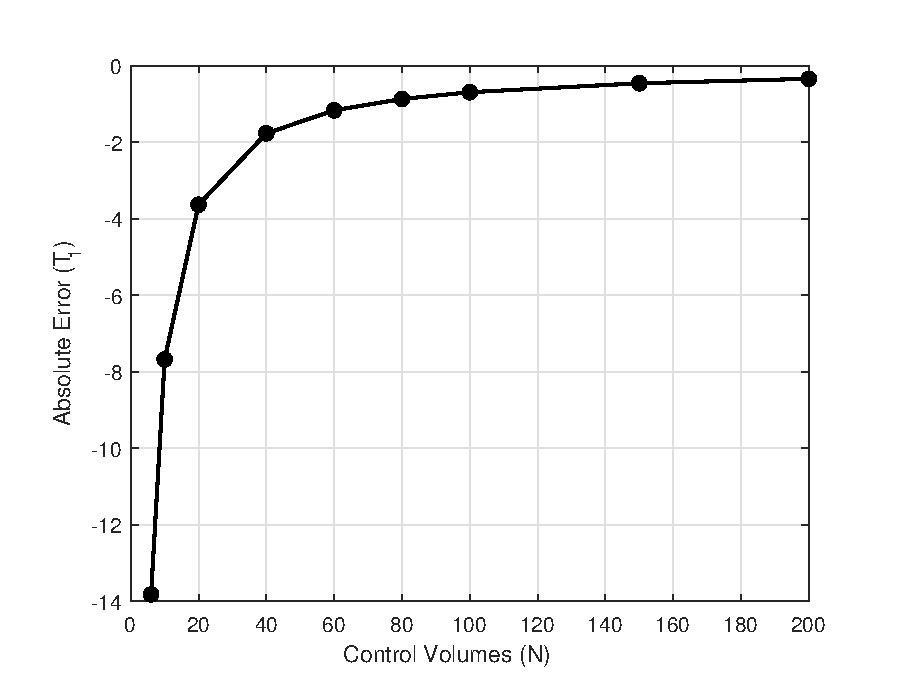
\includegraphics[scale=0.8]{error.eps}
    \caption{Absolute temperature error on the left border when varying the number of control volumes and using the linear variation of conductivity at the interface.}
    \label{fig:error}
\end{figure}
\section{Conclusion}

In this work, a program was implemented to solve a heat conduction problem in the steady state, through discretization by the finite volume method, in which the thermal conductivity at the interface between the two materials was evaluated by the resistance method and by linear variation .
The results showed that for the resistance method, the result obtained is exact, while for the linear variation, it is necessary to refine the mesh much more to obtain a temperature profile close to the real profile.


\end{document}
